%-=-=-=-=-=-=-=-=-=-=-=-=-=-=-=-=-=-=-=-=-=-=-=-=
%	DOCUMENT CLASS & PACKAGES
%-=-=-=-=-=-=-=-=-=-=-=-=-=-=-=-=-=-=-=-=-=-=-=-=

\documentclass[a4paper, 11pt]{article}

\usepackage{mhocolorthemenord}
\usepackage{mhomath}
\usepackage{mhotikz}
\usepackage{mhoworksheet}

%-=-=-=-=-=-=-=-=-=-=-=-=-=-=-=-=-=-=-=-=-=-=-=-=
%	BEGIN DOCUMENT
%-=-=-=-=-=-=-=-=-=-=-=-=-=-=-=-=-=-=-=-=-=-=-=-=

\begin{document}

\maketitle % Print the title section

%-=-=-=-=-=-=-=-=-=-=-=-=-=-=-=-=-=-=-=-=-=-=-=-=
%	SAGE SILENT 
%-=-=-=-=-=-=-=-=-=-=-=-=-=-=-=-=-=-=-=-=-=-=-=-=
\centering{\Huge{\cDarkGrey{Tao Unit Circle}}}

\vspace{2cm}
\begin{center}
\begin{tikzpicture}[scale=6.5]
 \draw[<->] (-1.25,0) -- (1.25,0) node[anchor=north] {\( x \)};
 \draw [<->](0,-1.25) -- (0,1.25) node[anchor=west] {\( y \)};
 \draw (0,0) circle (1cm);
 \draw[\cnBlue] (30:1cm) -- (0,0);
 \draw[\cnBlue] (45:1cm) -- (0,0);
 \draw[\cnBlue] (60:1cm) -- (0,0);

% 30 Degree Angle
\draw[\cnBlue] (30:1cm) -- (0,0);
\node[anchor=west, rotate=30] (a1) at  ({cos(30)},{sin(30)}) {\( \left(\frac{\sqrt{3}}{2}, \, \frac{1}{2} \right) \)};
\node[rotate=30, fill=white] (a2) at ({cos(30)*.5}, {sin(30)*.5}) {\footnotesize{\( 30^{\circ} \)}};
\node[rotate=30, fill=white] (a3) at ({cos(30)*.8}, {sin(30)*.8}) {\normalsize{\( \frac{\tau}{12} \)}};
\coordinate(a) at ({cos(30)},{sin(30)});
% 45 Degree Angle
\draw[\cnBlue] (45:1cm) -- (0,0);
\node[anchor=west, rotate=45] (b1) at  ({cos(45)},{sin(45)}) {\( \left(\frac{\sqrt{2}}{2}, \, \frac{\sqrt{2}}{2} \right) \)};
\node[rotate=45, fill=white] (b2) at ({cos(45)*.5}, {sin(45)*.5}) {\footnotesize{\( 45^{\circ} \)}};
\node[rotate=45, fill=white] (b3) at ({cos(45)*.8}, {sin(45)*.8}) {\normalsize{\( \frac{\tau}{8} \)}};
\coordinate(b) at ({cos(45)},{sin(45)});
% 60 Degree Angle
\draw[\cnBlue] (60:1cm) -- (0,0);
\node[anchor=west, rotate=60] (c1) at  ({cos(60)},{sin(60)}) {\( \left(\frac{1}{2} , \, \frac{\sqrt{3}}{2} \right) \)};
\node[rotate=60, fill=white] (c2) at ({cos(60)*.5}, {sin(60)*.5}) {\footnotesize{\( 60^{\circ} \)}};
\node[rotate=60, fill=white] (c3) at ({cos(60)*.8}, {sin(60)*.8}) {\normalsize{\( \frac{\tau}{6} \)}};
\coordinate(c) at ({cos(60)},{sin(60)});
% 90 Degree Angle
\node[anchor=west, above left] (d1) at  ({cos(90)},{sin(90)}) {\( \left(0 , \, 1 \right) \)};
\node[fill=white] (d2) at ({cos(90)*.5}, {sin(90)*.5}) {\footnotesize{\( 90^{\circ} \)}};
\node[fill=white] (d3) at ({cos(90)*.8}, {sin(90)*.8}) {\normalsize{\( \frac{\tau}{4} \)}};
\coordinate(d) at ({cos(90)},{sin(90)});
% 120 Degree Angle
\draw[\cnBlue] (120:1cm) -- (0,0);
\node[anchor=east, rotate=300] (e1) at  ({cos(120)},{sin(120)}) {\( \left(-\frac{1}{2} , \, \frac{\sqrt{3}}{2} \right) \)};
\node[rotate=300, fill=white] (e2) at ({cos(120)*.5}, {sin(120)*.5}) {\footnotesize{\( 120^{\circ} \)}};
\node[rotate=300, fill=white] (e3) at ({cos(120)*.8}, {sin(120)*.8}) {\normalsize{\( \frac{\tau}{3} \)}};
\coordinate(e) at ({cos(120)},{sin(120)});
% 135 Degree Angle
\draw[\cnBlue] (135:1cm) -- (0,0);
\node[anchor=east, rotate=315] (f1) at  ({cos(135)},{sin(135)}) {\( \left(-\frac{\sqrt{2}}{2} , \, \frac{\sqrt{2}}{2} \right) \)};
\node[rotate=315, fill=white] (f2) at ({cos(135)*.5}, {sin(135)*.5}) {\footnotesize{\( 135^{\circ} \)}};
\node[rotate=315, fill=white] (f3) at ({cos(135)*.8}, {sin(135)*.8}) {\normalsize{\( \frac{3 \tau}{8} \)}};
\coordinate(f) at ({cos(135)},{sin(135)});
% 150 Degree Angle
\draw[\cnBlue] (150:1cm) -- (0,0);
\node[anchor=east, rotate=330] (g1) at  ({cos(150)},{sin(150)}) {\( \left(-\frac{\sqrt{3}}{2} , \, \frac{1}{2} \right) \)};
\node[rotate=330, fill=white] (g2) at ({cos(150)*.5}, {sin(150)*.5}) {\footnotesize{\( 150^{\circ} \)}};
\node[rotate=330, fill=white] (g3) at ({cos(150)*.8}, {sin(150)*.8}) {\normalsize{\( \frac{5 \tau}{12} \)}};
\coordinate(g) at ({cos(150)},{sin(150)});
% 180 Degree Angle
\node[anchor=south, above left] (h1) at  ({cos(180)},{sin(180)}) {\( \left(-1 , \, 0 \right) \)};
\node[fill=white] (h2) at ({cos(180)*.5}, {sin(180)*.5}) {\footnotesize{\( 180^{\circ} \)}};
\node[fill=white] (h3) at ({cos(180)*.8}, {sin(180)*.8}) {\normalsize{\( \dfrac{\tau}{2} \)}};
\coordinate(h) at ({cos(180)},{sin(180)});
% 210 Degree Angle
\draw[\cnBlue] (210:1cm) -- (0,0);
\node[anchor=east, rotate=30] (i1) at  ({cos(210)},{sin(210)}) {\( \left(-\frac{\sqrt{3}}{2} , \, -\frac{1}{2} \right) \)};
\node[rotate=30, fill=white] (i2) at ({cos(210)*.5}, {sin(210)*.5}) {\footnotesize{\( 210^{\circ} \)}};
\node[rotate=30, fill=white] (i3) at ({cos(210)*.8}, {sin(210)*.8}) {\normalsize{\( \frac{7 \tau}{12} \)}};
\coordinate(i) at ({cos(210)},{sin(210)});
% 225 Degree Angle
\draw[\cnBlue] (225:1cm) -- (0,0);
\node[anchor=east, rotate=45] (j1) at  ({cos(225)},{sin(225)}) {\( \left(-\frac{\sqrt{2}}{2} , \, -\frac{\sqrt{2}}{2} \right) \)};
\node[rotate=45, fill=white] (j2) at ({cos(225)*.5}, {sin(225)*.5}) {\footnotesize{\( 225^{\circ} \)}};
\node[rotate=45, fill=white] (j3) at ({cos(225)*.8}, {sin(225)*.8}) {\normalsize{\( \frac{5 \tau}{8} \)}};
\coordinate(j) at ({cos(225)},{sin(225)});
% 240 Degree Angle
\draw[\cnBlue] (240:1cm) -- (0,0);
\node[anchor=east, rotate=60] (k1) at  ({cos(240)},{sin(240)}) {\( \left(-\frac{1}{2} , \, -\frac{\sqrt{3}}{2} \right) \)};
\node[rotate=60, fill=white] (k2) at ({cos(240)*.5}, {sin(240)*.5}) {\footnotesize{\( 240^{\circ} \)}};
\node[rotate=60, fill=white] (k3) at ({cos(240)*.8}, {sin(240)*.8}) {\normalsize{\( \frac{2\tau}{3} \)}};
\coordinate(k) at ({cos(240)},{sin(240)});
% 270 Degree Angle
\node[anchor=east, below right] (l1) at  ({cos(270)},{sin(270)}) {\( \left(0 , \, -1 \right) \)};
\node[fill=white] (l2) at ({cos(270)*.5}, {sin(270)*.5}) {\footnotesize{\( 270^{\circ} \)}};
\node[fill=white] (l3) at ({cos(270)*.8}, {sin(270)*.8}) {\normalsize{\( \frac{3\tau}{4} \)}};
\coordinate(l) at ({cos(270)},{sin(270)});
% 240 Degree Angle
\draw[\cnBlue] (300:1cm) -- (0,0);
\node[anchor=west, rotate=300] (m1) at  ({cos(300)},{sin(300)}) {\( \left(\frac{1}{2} , \, -\frac{\sqrt{3}}{2} \right) \)};
\node[rotate=300, fill=white] (m2) at ({cos(300)*.5}, {sin(300)*.5}) {\footnotesize{\( 300^{\circ} \)}};
\node[rotate=300, fill=white] (m3) at ({cos(300)*.8}, {sin(300)*.8}) {\normalsize{\( \frac{5\tau}{6} \)}};
\coordinate(m) at ({cos(300)},{sin(300)});
% 315 Degree Angle
\draw[\cnBlue] (315:1cm) -- (0,0);
\node[anchor=west, rotate=315] (n1) at  ({cos(315)},{sin(315)}) {\( \left(\frac{\sqrt{2}}{2} , \, -\frac{\sqrt{2}}{2} \right) \)};
\node[rotate=315, fill=white] (n2) at ({cos(315)*.5}, {sin(315)*.5}) {\footnotesize{\( 315^{\circ} \)}};
\node[rotate=315, fill=white] (n3) at ({cos(315)*.8}, {sin(315)*.8}) {\normalsize{\( \frac{7 \tau}{8} \)}};
\coordinate(n) at ({cos(315)},{sin(315)});
% 330 Degree Angle
\draw[\cnBlue] (330:1cm) -- (0,0);
\node[anchor=west, rotate=330] (o1) at  ({cos(330)},{sin(330)}) {\( \left(\frac{\sqrt{3}}{2} , \, -\frac{1}{2} \right) \)};
\node[rotate=330, fill=white] (o2) at ({cos(330)*.5}, {sin(330)*.5}) {\footnotesize{\( 330^{\circ} \)}};
\node[rotate=330, fill=white] (o3) at ({cos(330)*.8}, {sin(330)*.8}) {\normalsize{\( \frac{11 \tau}{12} \)}};
\coordinate(o) at ({cos(330)},{sin(330)});
% 360 Degree Angle
\node[anchor=south, above right] (p1) at  ({cos(0)},{sin(0)}) {\( \left(1 , \, 0 \right) \)};
\node[fill=white] (p2) at ({cos(0)*.5}, {sin(0)*.5}) {\footnotesize{\( 0^{\circ} \)}};
\node[fill=white] (p3) at ({cos(0)*.8}, {sin(0)*.8}) {\normalsize{\( \tau \)}};
\coordinate(p) at ({cos(0)},{sin(0)});
    \foreach \p in {a,b,c,d,e,f,g,h,i,j,k,l,m,n,o,p}
    \fill [opacity=.5] (\p) circle(.5pt);
\end{tikzpicture}
\end{center}
\customfootnosage
\end{document}

